\section{速度合成律的失效}\label{sec:02.06}

如图\ref{fig:02.10}~所示,如果在炮车上装有两门相同的大炮,一门向
右,一门向左。如果炮车相对地面静止\lhbrak 图\ref{fig:02.10a}\,\rhbrak,这时,不论
从地面参考系$K$,还是从炮车参考系$K'$看,同时向左、右发射出
的炮弹的速率都是$v$。如果炮车相对地面以$u$的速率向右匀速运动
\lhbrak 图\ref{fig:02.10b}\,\rhbrak ,从$K$看,按速度合成规律\lhbrak 式\eqref{eqn:02.03.06}\,\rhbrak ,向右的炮
弹速率是$v+u$;向左的炮弹速率是$v-u$。实验也相当精确地证
明了这一点,它表明,速度的合成公式是符合实际的。

我们现在要问:速度合成律对任何情况都成立吗?

\clearpage
\begin{figure}
    \centering
    \subfigure[]{
        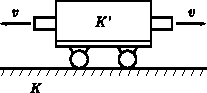
\includegraphics{figure/fig02.10a}
        \label{fig:02.10a}
    }
    \hspace{2em}
    \subfigure[]{
        \centering
        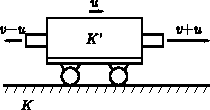
\includegraphics{figure/fig02.10b}
        \label{fig:02.10b}
    }
    \caption{速度的合成}
    \label{fig:02.10}
\end{figure}

\begin{figure}
    \centering
    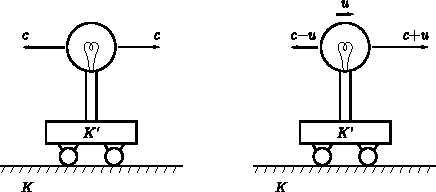
\includegraphics{figure/fig02.11}
    \caption{光的速度合成}
    \label{fig:02.11}
\end{figure}

再考虑一个如图\ref{fig:02.11}~所示的实验,这里仅把大炮改为灯泡,
灯泡发出的光与炮弹相当,光相对于灯泡的速率是$c$。根据速度合
成律,当灯泡相对于地面以速率$u$向右匀速运动时,则向右发出的
光对于地面参考系$K$的速率应是$c+u$,而向左发出的光对于$K$的
速率应是$c-u$。这个结果对吗?现在我们举一些显而易见的例
子,来说明这个结果是不正确的。

上述实验是把速度合成律应用到光传播的现象中去。根据光
学知识,我们知道,一个物体$A$之所以能被看到,是由于从物体
$A$发出的光(或从它反射的光)传到了我们的眼睛。例如,在图\ref{fig:02.12}~
中,1投球,2接球。2看到球$A$,是由于球$A$发出的光到达2。如果
光速为$c$,1到2之间距离为$L$,并且1即将投球的时刻为$t=0$,则
2看到1即将投球的时刻为
\begin{equation*}
    t_{2\text{投}}=\frac{L}{c}
\end{equation*}
\begin{figure}
    \centering
    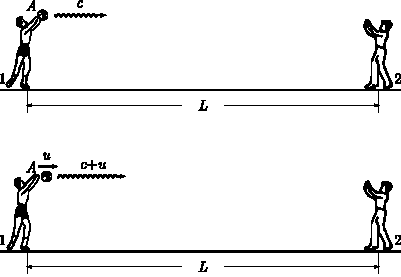
\includegraphics{figure/fig02.12}
    \caption{光的速度合成引起的混乱}
    \label{fig:02.12}
\end{figure}%
当1刚刚将球投出时,球$A$速率为$u$,如果光也满足速度合成律,
那么,这时球$A$发出的光相对于地面的速度应为$c+u$。如果1刚
刚将球投出的时刻是$t=t_{1\text{出}}$(即1投球这一动作所用的时间间隔),
则2看到1刚刚将球投出的时刻应为
\begin{equation*}
    t_{2\text{出}} = t_{1\text{出}} + \frac{L}{c+u}
\end{equation*}

从原则上讲。我们总有办法(譬如增大$L$)使下式成立
\begin{equation*}
    \frac{L}{c} > t_{1\text{出}} + \frac{L}{c+u}
\end{equation*}
亦即\vspace{-1.56em}
\begin{equation*}
    t_{2\text{投}} > t_{2\text{出}}
\end{equation*}
上式表明,2看到1开始投球的时刻比他看到1已经投出球的时刻
还要晚。更形象地说。2将先看到球$A$飞出,而后才看到1的投球
动作。这就是说,如果光的传播也满足速度合成公式\eqref{eqn:02.03.06},必然
导致先看到后发生的事,后看到先发生的事这种奇怪的现象,然
而,谁也没有见过这种现象。这说明光并不满足速度合成公式。

当然,有人会说,上述例子是假想实验,由于光速是很大
的,$L/c$或$L/\left(c+u\right)$实际上都接近于零,因而不可能观测到这种
现象。的确,在日常生活中涉及的速度与光速相比都是很小的,
把光速看成无限大,上述矛盾就没有了。但是,光速并不总能被
看成无限大,特别是在天体尺度上,光速不能被认为是无限大,光
传播中的矛盾是逃避不掉的。下面我们分析一个天文学上的真实
例子。

我国史书《宋史》中有下列的记载:“至和元年五月己丑出
天关东南可数寸岁余稍没”,《宋会要辑稿》也记载:“至和元
年五月晨出东方守天关昼见如太白芒角四出色赤白凡见二十三
日”。这个重要的天文观测记录说的是一次非常著名的超新星爆
发事件,现称为公元1054年的超新星。

所谓超新星指的是恒星在特定的演化阶段出现的一次大爆
发。原来发光很弱的星体,在爆发时,向外抛出速率很高的大量
物质,并发出很强的光,过不长的一段时间,又再暗下去。现在
巳确定,1054年超新星的遗迹就是金牛座中的蟹状星云,它到地
球的距离约为$L \approx 5000$光年,爆发时,喷射物的速率至少有
$u=1500$公里/秒。
\begin{figurex}
    \centering
    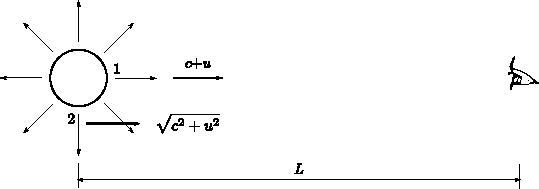
\includegraphics{figure/fig02.13}
    \caption{超新星爆发过程中光的传播}
    \label{fig:02.13}
\end{figurex}

由图\ref{fig:02.13}~看出,如果爆发时刻为$t=0$,且爆发时间极短,则
根据速度合成律,1处发出的传向观察者的光相对地面的速率是
$c+u$,所以观察者看到l发光的时刻是

\begin{equation*}
    t_{1}=\frac{L}{c+u} \approx \frac{L}{c}\left(1-\frac{u}{c}\right)
\end{equation*}
同样,根据速度合成律,2处(弧$\wideparen{12}=\ang{90;;}$)发出的传向观察者的光
相对于地面的速率约为$\sqrt{c^2 + u^2}$,故观察者看到2发光的时刻是
\begin{equation*}
    t_{2}=\frac{L}{\sqrt{c^{2}+u^{2}}} \approx \frac{L}{c}\left(1-\frac{1}{2} \cdot \frac{u^{2}}{c^{2}}\right)
\end{equation*}
显然,观察者见弧$\wideparen{12}$中发光的时刻介于$t_1$到$t_2$之间,因此观察者
看到星发光的时间至少应是
\begin{equation*}
    \Delta t=t_{2}-t_{1} \approx \frac{Lu}{c^{2}}
\end{equation*}
代入有关数据,计算而得
\begin{equation*}
    \Delta t=25\text{年}
\end{equation*}

如果爆发不作瞬时过程处理,则看到超新星的时间应比25年
还要长。

但是,这个下限与实际观测是不相符合的。记录上说:“凡
见二十三日”(白天看到)或“岁余稍没”(夜里看到)。即一年多
就消没了。

上述真实例子说明,对于光传播的现象,速度合成律是失效
的。它说明,从超新星不同地方发出的光,即不同光源发出的光,
相对于地面的速率之间的差别,不应有式\eqref{eqn:02.03.06}~所给出的那样
大。现代更精确的实验表明。光速是与光源速度无关的,无论光
源的速度有多么大,由它发出的光的速度仍与静止光源发出的光
的速度相同。这就是光速不变性,这个特点最初是由爱因斯坦注
意到的。

显然,光速不变性与速度合成律\lhbrak 式\eqref{eqn:02.03.06}\,\rhbrak 之间存在着严重
的矛盾,而问题的根源就在于伽利略变换并不总是适用的。